\documentclass[border=3pt]{standalone}
% Preâmbulo compartilhado pelos diagramas TikZ da aula 12 (Mapeamento por Grade de Ocupação)
\usepackage[T1]{fontenc}
\usepackage[utf8]{inputenc}
\usepackage{lmodern}
\usepackage{amsmath}
\usepackage{xcolor}
\usepackage{tikz}
\usetikzlibrary{arrows.meta,angles,quotes,decorations.pathmorphing,calc,
                positioning,shapes.geometric,shapes.misc,backgrounds,fit,
                math}

% Paleta (mesma dos SVGs originais)
\definecolor{dblue}{HTML}{2A5B8C}
\definecolor{dorange}{HTML}{B3541E}
\definecolor{dgreen}{HTML}{4A7C59}
\definecolor{dred}{HTML}{9C4B4B}
\definecolor{dcream}{HTML}{F4F1EA}
\definecolor{dshade}{HTML}{DDD7C9}

% Função gaussiana (não normalizada por padrão de escala visual)
\pgfmathdeclarefunction{gauss}{3}{%
  \pgfmathparse{1/(#3*sqrt(2*pi))*exp(-((#1-#2)^2)/(2*#3^2))}%
}

% Estilos comuns (prefixo d... para não colidir com chaves internas do pgf)
\tikzset{
  >={Stealth[length=2mm]},
  dguide/.style={gray!55, dashed, line width=0.4pt},
  daxis/.style={gray!60, line width=0.7pt, ->},
  dbody/.style={fill=black!3, draw=black!80, line width=1pt},
  dacc/.style={draw=dblue, line width=1pt},
  dlbl/.style={black!55, font=\small},
  dsub/.style={black!45, font=\footnotesize},
  dstate/.style={circle, draw=black!80, fill=dcream, line width=1pt,
                 minimum size=17mm, font=\large, inner sep=1pt},
  dobs/.style={circle, draw=black!80, fill=dshade, line width=1pt,
               minimum size=14mm, font=\large, inner sep=1pt},
  dbox/.style={rounded corners=2pt, draw=black!80, fill=dcream, line width=1pt,
               align=center, inner sep=6pt},
  dop/.style={circle, draw=black!80, fill=white, line width=1pt,
              minimum size=6mm, inner sep=0pt, font=\small},
  dtrans/.style={->, dblue, line width=1pt},
  dmeas/.style={->, dorange, line width=1pt},
  dcurve/.style={line width=1pt, dblue},
  dcurveb/.style={line width=1.4pt, dorange},
}

\begin{document}
\hyphenpenalty=10000 \exhyphenpenalty=10000 \tolerance=9999 \emergencystretch=3em
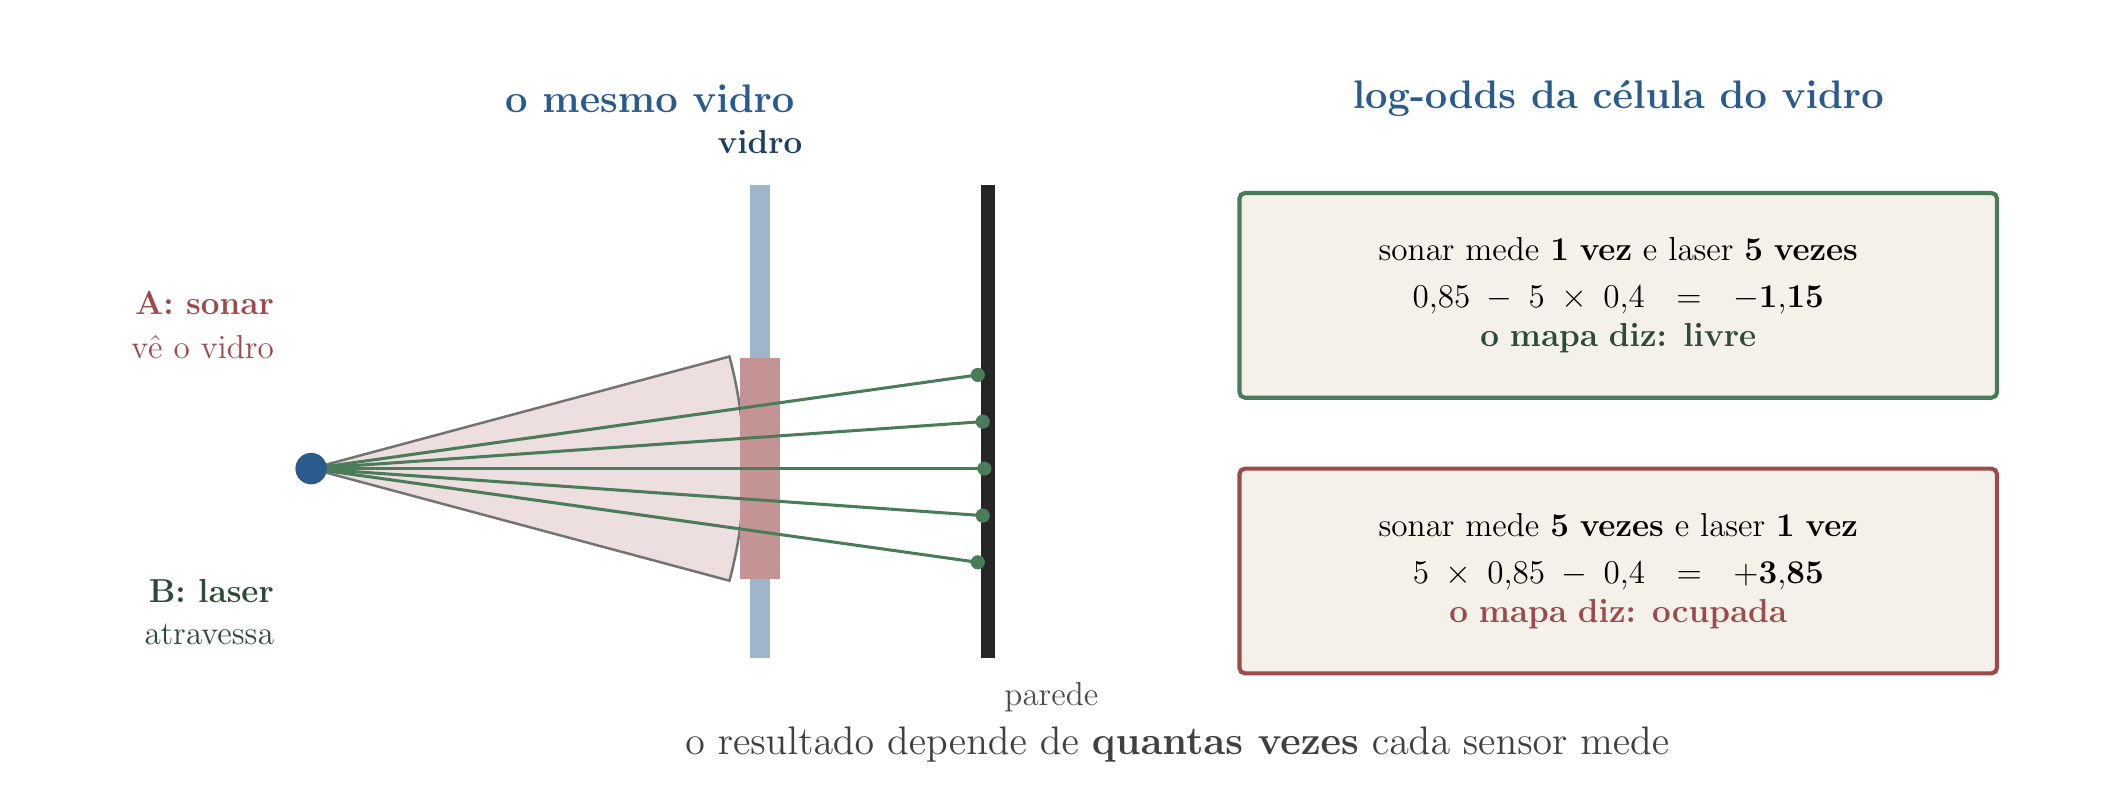
\begin{tikzpicture}[x=1cm,y=1cm]
  \useasboundingbox (-3.6,-3.9) rectangle (22.4,5.6);
  % ---- cena (vista de cima) ----
  \node[font=\Large\bfseries, dblue] at (4.3,4.7) {o mesmo vidro};
  \draw[black!85, line width=5pt] (8.6,-2.4) -- (8.6,3.6);
  \node[font=\large, black!70] at (9.4,-2.9) {parede};
  \draw[dblue!45, line width=7pt, line cap=butt] (5.7,-2.4) -- (5.7,3.6);
  \node[font=\large\bfseries, dblue!70!black] at (5.7,4.15) {vidro};
  % sonar (A): cone largo que para no vidro
  \fill[dred!18] (0,0) -- (-15:5.5) arc(-15:15:5.5) -- cycle;
  \draw[black!55, line width=0.9pt] (0,0) -- (-15:5.5) arc(-15:15:5.5) -- cycle;
  \fill[dred!60] (5.45,-1.4) rectangle (5.95,1.4);
  % laser (B): feixes finos que atravessam o vidro
  \foreach \a in {-8,-4,0,4,8} {\draw[dgreen, line width=1.1pt] (0,0) -- (\a:8.55);}
  \foreach \a in {-8,-4,0,4,8} {\fill[dgreen] (\a:8.55) circle (0.09);}
  \fill[dblue] (0,0) circle (0.2);
  \node[font=\large\bfseries, dred, anchor=east] at (-0.35,2.1) {A: sonar};
  \node[font=\large, dred, anchor=east] at (-0.35,1.55) {vê o vidro};
  \node[font=\large\bfseries, dgreen!60!black, anchor=east] at (-0.35,-1.55) {B: laser};
  \node[font=\large, dgreen!60!black, anchor=east] at (-0.35,-2.1) {atravessa};
  % ---- dois cenários para a mesma célula ----
  \node[font=\Large\bfseries, dblue] at (16.6,4.7) {log-odds da célula do vidro};
  \tikzset{c/.style={dbox, text width=9.2cm, minimum height=2.6cm, font=\large, line width=1.5pt, align=center}}
  \node[c, draw=dgreen] at (16.6,2.2) {sonar mede \textbf{1 vez} e laser \textbf{5 vezes}\\[3pt] $0{,}85 - 5 \times 0{,}4 = \mathbf{-1{,}15}$\\ \textbf{\textcolor{dgreen!60!black}{o mapa diz: livre}}};
  \node[c, draw=dred] at (16.6,-1.3) {sonar mede \textbf{5 vezes} e laser \textbf{1 vez}\\[3pt] $5 \times 0{,}85 - 0{,}4 = \mathbf{+3{,}85}$\\ \textbf{\textcolor{dred}{o mapa diz: ocupada}}};
  \node[font=\Large, black!75] at (11.0,-3.5) {o resultado depende de \textbf{quantas vezes} cada sensor mede};
\end{tikzpicture}
\end{document}
